%************************************************
\chapter{Spring Boot and Cloud Frameworkt}\label{ch:spring}
%************************************************
Report and prototype requirements - topics to be covered

Topic 1: Write a brief introduction to the Spring Boot and Cloud Frameworks. Design, develop, test, and document a functional proof-of-concept prototype using the Spring Boot and Cloud Framework. The prototype should be able to:
\begin{itemize}
\item be configured remotely, so that every client fetches configuration at boot-time from a central configuration server
\item contain a simple graphical user interface
\item leverage the gateway API pattern to distribute requests to specific services
\item contain at least three data delivering services 
\end{itemize}
Microservices is a new architectural style that aims to realize software systems as a package of small services, each deployable on different platform. Every single Microservice has its own process while communicating with other services via lightweight mechanisms like RESTFull APIs.\\

All the services has business capability which can utilize various programming languages and data stores. A system has a microservices architecture when that system is composed of several services without any centralized control.\\

Resilience to failure is another characteristic of microservices as every request in this new setting gets translated to several service calls through the system. To have a fully functional microservices architecture and to take advantage of all of its benefits, the following components have to be utilized. Most of these components addresses the complexities of distributing the business logic among the services:

\begin{itemize}
	\item Configuration Server: It is one of the principles of Continuous Delivery to decouple source code from its configuration. It enables us to change the configuration of our application without redeploying the code. As a microservices architecture have so many services, and their re-deployment is going to be costly, it is better to have a configuration server so that the services could fetch their corresponding configurations.
	\item Service Discovery: 
	In a microservices architecture, there exist several services that each of them might have many instances in order to scale themselves to the underlying load. Thus, keeping track of the deployed services, and their exact address and port number is a cumbersome task. The solution is to use a Service Discovery component in order to get the available instances of each service.		
\end{itemize}

\textbf{What is Spring Cloud?}\\
The Spring Cloud Framework provides an implementation of many of the different patterns used for building distributed systems. Spring Cloud builds on some common elements from the Spring Framework and Spring Boot Framework. Spring Cloud provides tools to some of the most common patterns in distributed systems such it is easier for developers to build these patterns. It provides among other tools for configuration management, service discovery, intelligent routing, Load balancing and much more patterns.\\

\textbf{What is Spring Boot?}\\
The Spring Boot Framework makes it easy to deploy and run Spring based applications. Spring Boot can with minimal Spring configuration create and run a \eg Spring Cloud based application in java.  \\
%ref: http://www.kennybastani.com/2015/07/spring-cloud-docker-microservices.html 


\section{Spring Boot and Cloud Framework PoC}
\begin{itemize}
	\item be configured remotely, so that every client fetches configuration at boot-time from a central configuration server
	\item contain a simple graphical user interface
	\item leverage the gateway API pattern to distribute requests to specific services
	\item contain at least three data delivering services 
\end{itemize}

For creating a Microservice based on Spring Cloud we generate a Spring Boot project with the necessary dependencies using the \emph{Spring Initializr}\footnote{https://start.spring.io/}. For this project the dependency ``Web'' is used which among others contains Tomcat and Spring MVC libraries. We use the Spring MVC libraries to be able to create a graphical view for the user. This graphical user interface is created with HTML using the \emph{Thymeleaf} template by including the necessary dependency in the Maven POM-file, see listing \ref{lst:thymeleaf}. 
\begin{lstlisting}[caption={Thymeleaf dependency in POM-file},label={lst:thymeleaf}, language=XML, frame=single, ]
<dependency>
	<groupId>org.springframework.boot</groupId>
	<artifactId>spring-boot-starter-thymeleaf</artifactId>
</dependency>
\end{lstlisting}
After building the microservices with a graphical user interface, it is necessary to setup Spring Cloud Config.
First a Spring Boot project for the configuration server is generated from the Spring Initializr based on the Config Server dependency from Spring Cloud. As shown on figure \ref{fig:cloud-config} the Config Server is connected to a git repository. The git repository contains the configuration files which are loaded by the Config Server. In each service a Spring Cloud Config Client service is implemented such the services are able to adapt the configurations which the Config Server gets from the git repository.  
\begin{figure}[bth]
	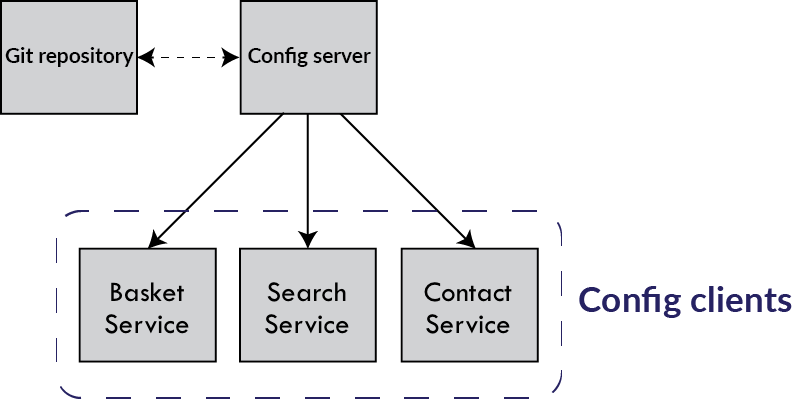
\includegraphics[width=1\linewidth]{gfx/cloud-config}
	\caption[cloudconfig]{Cloud configuration} \label{fig:cloud-config}
\end{figure}    

The API Gateway Pattern helps minimizing the number of requests made to the backend of the services.
The API Gateway is implemented in the Homepage service see figure \ref{fig:homepage-yml}.  
\begin{figure}[bth]
	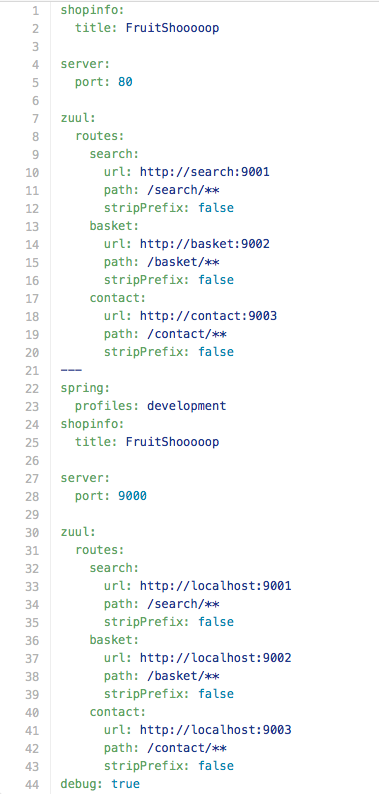
\includegraphics[width=0.6\linewidth]{gfx/homepage-yml}
	\caption[homepageyml]{Homepage yaml file} \label{fig:homepage-yml}
\end{figure}    

